\documentclass[]{article}

\usepackage[margin=1in]{geometry}
\usepackage{physics}
\usepackage{amsmath}
\usepackage{graphicx}


%opening
\title{SYSM 6302 - Lab 7\\
Dynamical Systems \& Stability}
\author{Jonas Wagner}
\date{2021 May 25}

\begin{document}
	

\maketitle

\newpage
\section*{Phase Plane Portraits of Linear System}

For each of the linear systems below:
\begin{enumerate}
	\item Determine the state matrix $A$, for $\dot{x} = A x$
	\item Classify the equilibrium $x = 0$ by examining the eigenvalues of $A$. Compute the eigenvalues by hand – you can check your answers with a computer/calculator.
	\item Use a phase plane plottler to plot phase plane portraits. If the eigenvectors of A are real, draw them on top of the corresponding phase plane portrait. Compute the eigenvectors by hand for problems 2 and 4, the rest use a computer program. On all plots, pick 4 points (not along the eigenvectors) and plot an arrow in the direction of the vector field $f = \mqty(f_1\\ f_2) = \mqty(\dot{x}_1\\ \dot{x}_2)$
\end{enumerate}



\section{Problem 1:}
\begin{align*}
	\dot{x}_1 &= x_2\\
	\dot{x}_2 &= x_1 - x_2
\end{align*}

\subsection{Part a}
\begin{displaymath}
	A = \mqty[0&1\\1&-1]
\end{displaymath}

\subsection{Part b}

\begin{align*}
	(sI - A)
	&= \mqty[s & -1\\ -1 & s+1]\\
	\det(sI-A)
	&= s(s+1) - (-1)(-1)\\
	&= s^2 + s - 1\\
	\lambda_{1,2}
	&= \cfrac{-1 \pm \sqrt{1 - 4(1)(-1)}}{2(1)}\\
	&= -\frac{1}{2} \pm \frac{\sqrt{5}}{2}\\
	\lambda_1
	&= \frac{-1 + \sqrt{5}}{2} \approx 0.61803\\
	\lambda_2
	&= \frac{-1 - \sqrt{5}}{2} \approx -1.618
\end{align*}

\subsection{Part c}

\begin{align*}
	v_1 &= \mqty(-1 + \cfrac{\sqrt{5}}{2}\\ 2)\\
	v_2 &= \mqty(-1 - \cfrac{\sqrt{5}}{2}\\ 2)
\end{align*}

\begin{figure}[p]
	\centering
	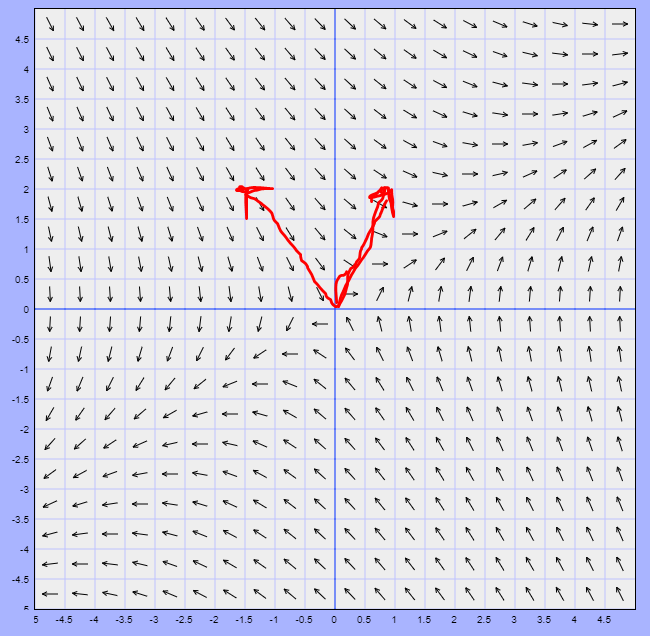
\includegraphics[width=0.7\linewidth]{fig/pblm1_w_vectors}
	\caption{Phase plane portrait of problem 1}
	\label{fig:pblm1}
\end{figure}


\newpage
\section{Problem 2:}
\begin{align*}
	\dot{x}_1 &= x_2\\
	\dot{x}_2 &= -3 x_1 - 4 x_2
\end{align*}

\subsection{Part a}
\begin{displaymath}
	A = \mqty[0&1\\-3&-4]
\end{displaymath}

\subsection{Part b}

\begin{align*}
	(sI - A)
	&= \mqty[s & -1\\ 3 & s+4]\\
	\det(sI-A)
	&= s(s+4) - (3)(-1)\\
	&= s^2 + 4s + 3\\
	&= (s + 1) (s + 3)\\
	\lambda_1
	&= -1\\
	\lambda_2
	&= -3
\end{align*}

\subsection{Part c}

\begin{align*}
	A v_1
	&= \lambda_1 v_1\\
	\mqty[0&1\\-3&-4] \mqty[a\\b]
	&= (-1) \mqty[a\\b]\\
	b &= -a\\
	-3 a - 4 b &= -b\\
	-3a &= 3b\\
	v_1 &= \mqty[1\\ -1] \text{ or }  \mqty[\cfrac{1}{\sqrt{2}}\\ -\cfrac{1}{\sqrt{2}}]
\end{align*}


\begin{align*}
	A v_2
	&= \lambda_1 v_2\\
	\mqty[0&1\\-3&-4] \mqty[a\\b]
	&= (-3) \mqty[a\\b]\\
	b &= -3a\\
	-3 a - 4 b &= -3b\\
	-3a &= b\\
	v_1 &= \mqty[1\\ -3] \text{ or } \mqty[\cfrac{1}{\sqrt{10}}\\ -\cfrac{3}{\sqrt{10}}]
\end{align*}


\begin{figure}[p]
	\centering
	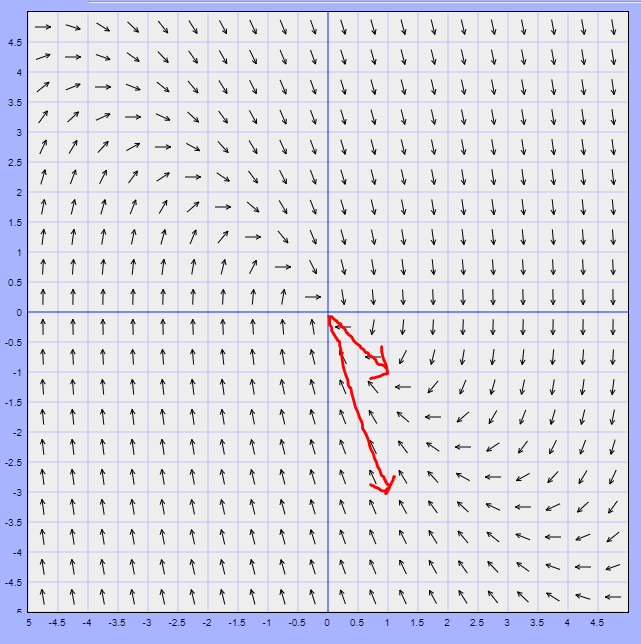
\includegraphics[width=0.7\linewidth]{fig/pblm2_w_vectors}
	\caption{Phase plane portrait of problem 2}
	\label{fig:pblm2}
\end{figure}


\newpage
\section{Problem 3:}
\begin{align*}
	\dot{x}_1 &= x_2\\
	\dot{x}_2 &= -4 x_1 - 2 x_2
\end{align*}

\subsection{Part a}
\begin{displaymath}
	A = \mqty[0&1\\-4&-2]
\end{displaymath}

\subsection{Part b}

\begin{align*}
	(sI - A)
	&= \mqty[s & -1\\ 4 & s+2]\\
	\det(sI-A)
	&= s(s+2) - (4)(-1)\\
	&= s^2 + 2 s + 4\\
	\lambda_{1,2}
	&= \cfrac{-2 \pm \sqrt{2 - 4(1)(4)}}{2(1)}\\
	&= -1 \pm j\frac{\sqrt{14}}{2}
\end{align*}

\subsection{Part c}

\begin{align*}
	v_1 &= \mqty(-1 - j \sqrt{3}\\ 4)\\
	v_2 &= \mqty(-1 + j \sqrt{3}\\ 4)
\end{align*}

\begin{figure}[p]
	\centering
	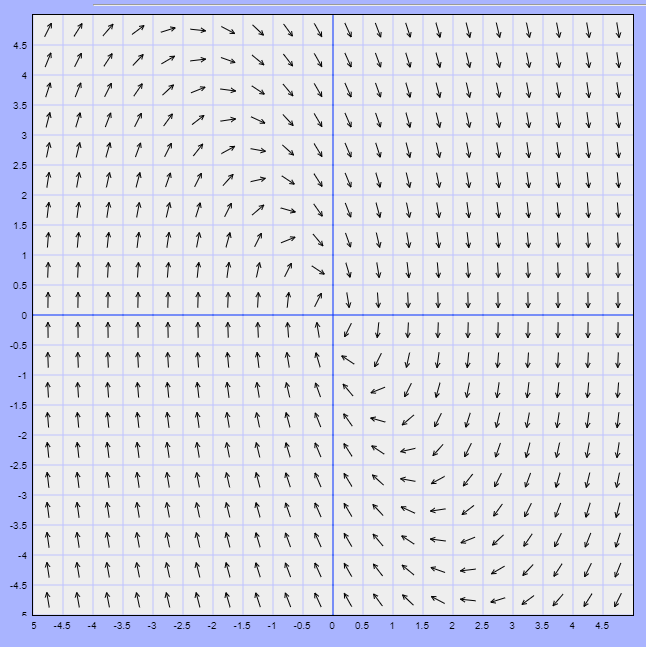
\includegraphics[width=0.7\linewidth]{fig/pblm3}
	\caption{Phase plane portrait of problem 3}
	\label{fig:pblm3}
\end{figure}


\newpage
\section{Problem 4:}
\begin{align*}
	\dot{x}_1 &= x_2\\
	\dot{x}_2 &= - 2 x_1 + 3 x_2
\end{align*}

\subsection{Part a}
\begin{displaymath}
	A = \mqty[0&1\\-2&3]
\end{displaymath}

\subsection{Part b}

\begin{align*}
	(sI - A)
	&= \mqty[s & -1\\ 2 & s-3]\\
	\det(sI-A)
	&= s(s-3) - (2)(-1)\\
	&= s^2 -3s + 2\\
	&= (s - 1) (s - 2)\\
	\lambda_1
	&= 1\\
	\lambda_2
	&= 2
\end{align*}

\subsection{Part c}


\begin{align*}
	A v_1
	&= \lambda_1 v_1\\
	\mqty[0&1\\-2&3] \mqty[a\\b]
	&= (1) \mqty[a\\b]\\
	b &= a\\
	-2 a +3 b &= b\\
	-2a &= -2b\\
	v_1 &= \mqty[1\\ 1] \text{ or }  \mqty[\cfrac{1}{\sqrt{2}}\\ \cfrac{1}{\sqrt{2}}]
\end{align*}


\begin{align*}
	A v_2
	&= \lambda_1 v_2\\
	\mqty[0&1\\-2&3] \mqty[a\\b]
	&= (2) \mqty[a\\b]\\
	b &= 2a\\
	-2 a +3 b &= 2b\\
	-2a &= -b\\
	v_2 &= \mqty[1\\ 2] \text{ or }  \mqty[\cfrac{1}{\sqrt{5}}\\ \cfrac{2}{\sqrt{5}}]
\end{align*}



\begin{figure}[p]
	\centering
	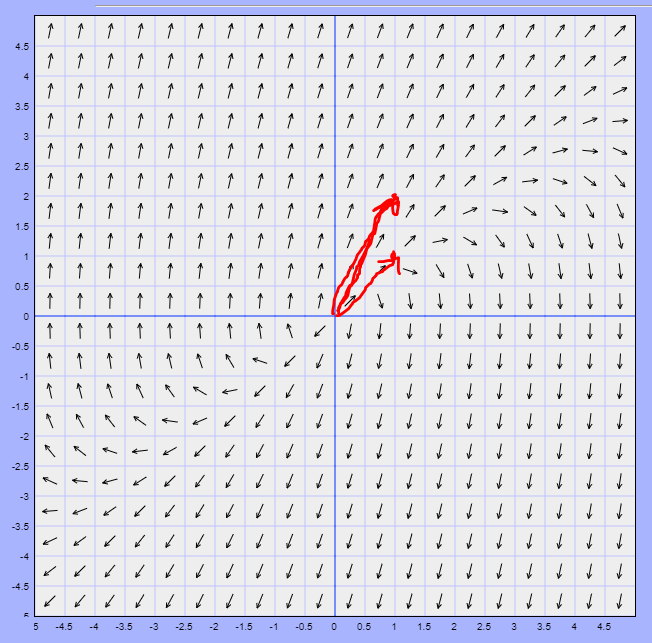
\includegraphics[width=0.7\linewidth]{fig/pblm4_w_vectors}
	\caption{Phase plane portrait of problem 4}
	\label{fig:pblm4}
\end{figure}


\newpage
\section{Problem 5:}
\begin{align*}
	\dot{x}_1 &= - x_1 + x_2\\
	\dot{x}_2 &= - 2 x_1 + x_2
\end{align*}

\subsection{Part a}
\begin{displaymath}
	A = \mqty[-1&1\\-2&1]
\end{displaymath}

\subsection{Part b}

\begin{align*}
	(sI - A)
	&= \mqty[s+1 & -1\\ 2 & s-1]\\
	\det(sI-A)
	&= (s+1)(s-1) - (2)(-1)\\
	&= s^2 -1 + 2\\
	&= s^2 + 1\\
	\lambda_{1,2}
	&= \pm j
\end{align*}

\subsection{Part c}


\begin{align*}
	v_1
	&= \mqty[1-j\\2]\\
	v_2
	&= \mqty[1+j\\2]
\end{align*}



\begin{figure}[p]
	\centering
	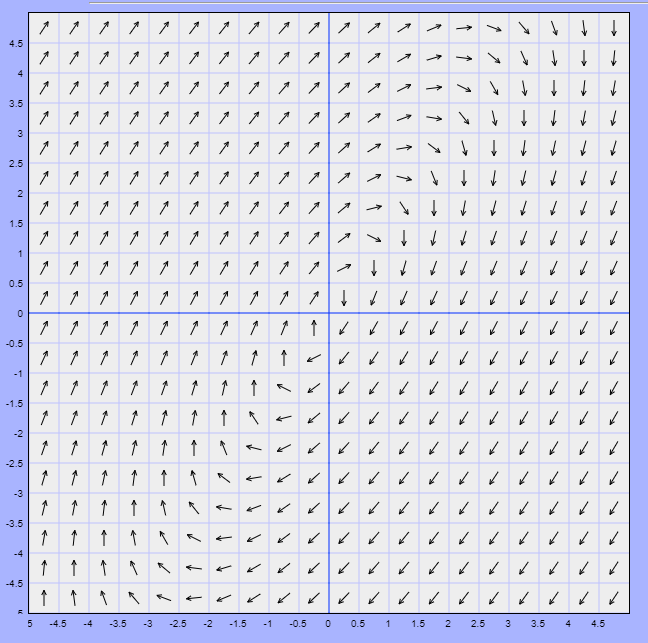
\includegraphics[width=0.7\linewidth]{fig/pblm5}
	\caption{Phase plane portrait of problem 5}
	\label{fig:pblm5}
\end{figure}




\section{Problem 6:}
Describe how the eigenvectors provide information about the shape of the phase plane portrait.\\

Eigenvectors themselves indicate the direction of each mode of the system associated with each eigenvalue. In the context of the phase plane portrait, eigenvectors can indicate important directions that relate the two state variables. This may be pointing in the direction of a particular asymptotic boundary or even a line in which the curl or divergence is equal to zero.




\newpage
\section*{Linearization of Nonlinear Systems}
For each of the nonlinear systems below:
\begin{enumerate}
	\item Identify the equilibrium points.
	\item Linearize the system around each of the equilibrium points.
	\item Classify the behavior of the linearized system around each equilibrium point.
\end{enumerate}

\section{Problem 7:}














	
\end{document}
